\documentclass{article}

\usepackage{microtype}
\usepackage{graphicx}
\usepackage{subcaption}
\usepackage{booktabs}
\usepackage{multirow}
\usepackage{hyperref}
\newcommand{\theHalgorithm}{\arabic{algorithm}}
\usepackage[preprint]{icml2026}
\usepackage{amsmath}
\usepackage{amssymb}
\usepackage{mathtools}
\usepackage[capitalize,noabbrev]{cleveref}
\usepackage{tikz}
\usetikzlibrary{positioning,arrows.meta,fit,backgrounds}
\usepackage{pgfplots}
\pgfplotsset{compat=1.18}
\usepackage{xspace}

\newcommand{\wev}{\textsc{wev}\xspace}

\icmltitlerunning{wev: Distilling LLM Browser Agents into Open System-One Decision Models}

\begin{document}

\twocolumn[
  \icmltitle{wev: Distilling LLM Browser Agents into\\Open, Local System-One Decision Models}

  \icmlsetsymbol{equal}{*}
  \begin{icmlauthorlist}
    \icmlauthor{AUTHOR NAME}{aff}
  \end{icmlauthorlist}
  \icmlaffiliation{aff}{AFFILIATION}
  \icmlcorrespondingauthor{AUTHOR NAME}{EMAIL}
  \icmlkeywords{decision models, browser agents, distillation, calibration}
  \vskip 0.3in
]

\printAffiliationsAndNotice{}

\begin{abstract}
System-One decision models answer typed questions about a free-form state with a probability for every declared
option, in one forward pass and without generating text, but the open models of this kind are trained on general
decision data and reach at most 21\% step success on browser steps from unseen websites. We observe that the typed
interface between a browser agent and its System One is itself a source of supervision: a prompted LLM placed behind it
while the agent works on live websites produces training data in exactly the decision model's format, and an LLM judge
reading each episode's final page decides which episodes to keep. We combine this interface distillation with Mind2Web
and NNetNav demonstrations converted to the same format, after auditing NNetNav's stopping labels, and with general
decision corpora. The resulting open models, \wev-1.7b, \wev-4b and \wev-8b, build on Qwen3 base models. \wev-4b
answers 76\% of browser steps on unseen websites correctly and stays competitive on general decision benchmarks. As the
System One of an open browser agent, it completes as many held-out live-website tasks as its LLM teacher, at
15--320\,ms per decision on one consumer GPU.
\end{abstract}

\section{Introduction}
\label{sec:intro}

Language-model agents act on the web by reading a page and choosing what to do next
\citep{yao2023react,zhou2024webarena,deng2023mind2web,he2024webvoyager}. Most of their steps do not require writing:
they require a choice among a small set of operations and, for the chosen operation, a choice among the elements on
the page. Generative LLMs make these choices by producing text that must then be parsed, which costs a full
autoregressive call per step and leaves the confidence of the choice implicit. System-One decision models
\citep{typesafe2026jev} replace this with a typed interface: the caller declares questions and their options at request
time, and the model returns a probability for every option in one forward pass, with nothing to parse and nothing that
can be malformed. The open agent jev-ultrafast \citep{jevultrafast2026} is built on this interface: at each step it asks
a hosted System One which operation to perform and which listed element to target.

Open decision models have followed quickly. Kev \citep{kev2026} adapts Qwen base models with LoRA and a pointer head,
Laya \citep{laya2026} fine-tunes ModernBERT \citep{warner2024modernbert}, and this-that-model \citep{cheng2026thisthat}
reads a 2B model's answer from a designated position; work on selective control \citep{wu2026reflex} and on read-out
failure modes \citep{sun2026typesafe} studies how such models behave inside agents. All of these models learn from
general decision data, meaning classification, question answering and rule records with short states. A browser step
is different in kind. Its state is a page of text and a list of 8--40 candidate elements, about 3{,}200 tokens in our
data, and its answer is grounded in that page rather than in world knowledge or in a rubric. Scored on identical
requests, Kev-4B and Kev-8B get 21\% and 19\% of steps on unseen websites fully right and Laya under 1\%
(\cref{sec:results-browser}).

The obstacle to closing this gap is supervision. Web demonstrations exist \citep{deng2023mind2web,murty2024nnetnav,lu2024weblinx},
but they are recorded in other action formats, they rarely contain the stopping and blocking decisions an agent needs,
and the stopping labels they do contain can be wrong. Collecting new human demonstrations in the decision format is
slow. Our key observation is that the decision interface itself makes supervision cheap: if a prompted LLM answers the
agent's typed requests while the agent works on live websites, every logged request--answer pair is already a training
example in the student's input and output format, with no translation between action spaces. What remains is to decide
which episodes to trust, and an LLM judge \citep{zheng2023judging} that reads the final page can make that decision.
We call this procedure \emph{interface distillation}.

We build \wev on this observation. A decision model following Kev's design is trained on three sources: episodes
from interface distillation with qwen3-max \citep{yang2025qwen3} as the teacher; Mind2Web and NNetNav steps converted
to the agent's request format, with NNetNav's stopping labels audited by a judge; and public general decision corpora
that keep the model a general-purpose System One. Our contributions are:
\begin{itemize}
\item We show that open System-One models trained on general decision data do not transfer to browser steps, and
release a conversion of Mind2Web and NNetNav into the request format of an open browser agent, with a single scorer
for decision models (\cref{sec:results-browser}).
\item We introduce interface distillation, which turns an LLM-backed agent run on live websites into judge-verified
training data for a non-generative decision model, and an audit of NNetNav's stopping labels that overturns 31\% of
its DONE labels (\cref{sec:method}).
\item We release \wev-1.7b, \wev-4b and \wev-8b. They reach 76\% step success on unseen websites, stay competitive on
general decision benchmarks, match their teacher's task success on 153 held-out live-website tasks, and answer in
15--320\,ms on one consumer GPU (\cref{sec:results}).
\end{itemize}
Code, data builders, models and per-request evaluation outputs are public.

\begin{figure*}[t]
\centering
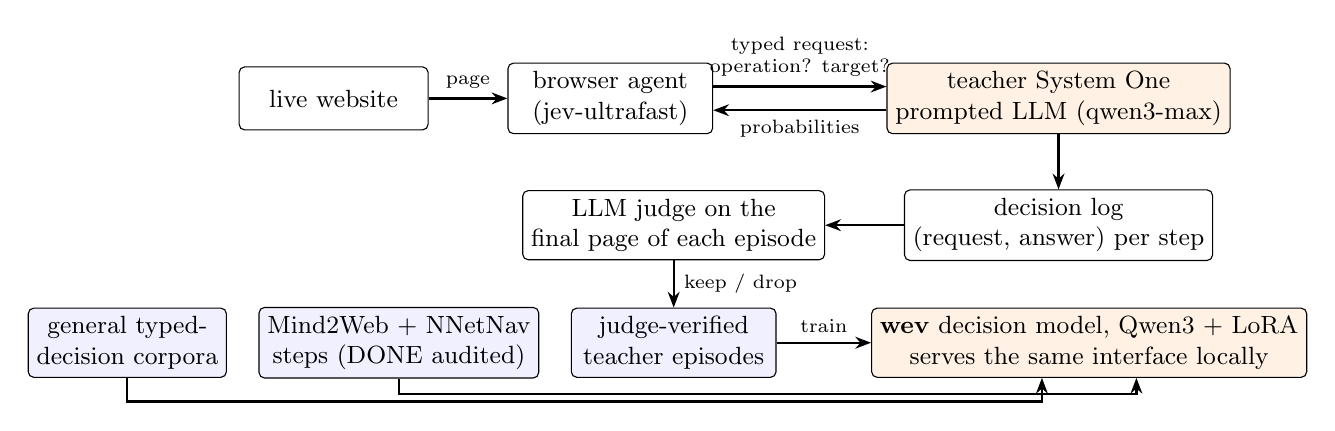
\begin{tikzpicture}[
  font=\small,
  box/.style={draw, rounded corners=2pt, align=center, minimum height=8mm, inner sep=3pt, fill=white},
  src/.style={box, fill=blue!6},
  mdl/.style={box, fill=orange!10},
  arr/.style={-{Stealth[length=2mm]}, thick},
  lab/.style={font=\scriptsize, align=center}
]
\node[box, minimum width=24mm] (web) {live website};
\node[box, right=10mm of web, minimum width=26mm] (agent) {browser agent\\(jev-ultrafast)};
\node[mdl, right=22mm of agent, minimum width=30mm] (teacher) {teacher System One\\prompted LLM (qwen3-max)};
\node[box, below=7mm of teacher, minimum width=30mm] (log) {decision log\\(request, answer) per step};
\node[box, left=10mm of log, minimum width=26mm] (judge) {LLM judge on the\\final page of each episode};
\node[src, below=6mm of judge, minimum width=26mm] (teach) {judge-verified\\teacher episodes};
\node[src, left=4mm of teach, minimum width=27mm] (demo) {Mind2Web + NNetNav\\steps (DONE audited)};
\node[src, left=4mm of demo, minimum width=24mm] (gen) {general typed-\\decision corpora};
\node[mdl, right=12mm of teach, minimum width=30mm] (student) {\textbf{\wev} decision model, Qwen3 + LoRA\\serves the same interface locally};
\draw[arr] (web) -- node[lab, above]{page} (agent);
\draw[arr] (agent.east) ++(0,1.5mm) -- node[lab, above]{typed request:\\operation? target?} ++(22mm,0);
\draw[arr] (teacher.west) ++(0,-1.5mm) -- node[lab, below]{probabilities} ++(-22mm,0);
\draw[arr] (teacher) -- (log);
\draw[arr] (log) -- (judge);
\draw[arr] (judge) -- node[lab, right]{keep / drop} (teach);
\draw[arr] (teach) -- node[lab, above]{train} (student);
\draw[arr] (gen.south) |- ++(0,-3mm) -| ([xshift=-6mm]student.south);
\draw[arr] (demo.south) |- ++(0,-2mm) -| ([xshift=6mm]student.south);
\end{tikzpicture}
\caption{Interface distillation. A browser agent sends typed requests to a System One served by a prompted LLM while
it works on live websites; every request and answer is logged in the decision model's own format, and an LLM judge
reading each episode's final page decides which episodes are kept. The student \wev trains on these episodes together
with converted demonstrations and general decision corpora, and then serves the same interface locally.}
\label{fig:overview}
\end{figure*}

\section{Related Work}
\label{sec:related}

\paragraph{System-One decision models.}
The hosted Jev model \citep{typesafe2026jev} introduced a model class that returns typed, calibrated answers instead
of text; its training method is unpublished. Open models share its interface but differ in backbone and data. Kev
\citep{kev2026} attaches LoRA adapters \citep{hu2022lora} and a pointer head to Qwen base models and trains on ten
public classification sources plus rule-composition records; Laya \citep{laya2026} fine-tunes a bidirectional encoder
\citep{devlin2019bert,warner2024modernbert} with a small decision head; this-that-model \citep{cheng2026thisthat} reads
answers from a designated position of a 2B decoder. REFLEX \citep{wu2026reflex} places a hosted decision model inside an
LLM agent and escalates to a strong LLM when confidence is low, and \citet{sun2026typesafe} show that decision heads can
follow an option's name rather than the rubric bound to it. None of these trains or evaluates a decision model on
browser steps, and none derives training data from an agent's own decision traffic.

\paragraph{Web agents and web data.}
Benchmarks for web agents range from simulated environments \citep{liu2018miniwob,yao2022webshop} to self-hosted
websites \citep{zhou2024webarena,koh2024visualwebarena} and live websites \citep{he2024webvoyager}. Mind2Web
\citep{deng2023mind2web} and WebLINX \citep{lu2024weblinx} record human demonstrations on real sites, and NNetNav
\citep{murty2024nnetnav} collects trajectories through unsupervised interaction with live sites. Most agents built on
these resources generate actions with an LLM \citep{yao2023react,zheng2024seeact,gur2024realworld}. We instead cast each
step as typed questions and answer them with a non-generative model, converting these resources into that format.

\paragraph{Distilling agents into smaller models.}
Knowledge distillation \citep{hinton2015distilling} and rationale distillation \citep{hsieh2023distilling} transfer
behaviour from large to small models, and agent fine-tuning on LLM-generated trajectories improves small generative
agents \citep{chen2023fireact,zeng2024agenttuning,schick2023toolformer}. Imitation learning from a queryable expert
\citep{ross2011dagger} motivates collecting labels on the learner's own state distribution. Interface distillation
differs in its target and its supervision channel: the student generates nothing, and the teacher is observed through
the same typed interface the student will serve, so the logged traffic needs no conversion.

\paragraph{Calibration, option bias and routing.}
Decision models are useful to the extent that their probabilities can be acted on. Modern networks are often
miscalibrated \citep{guo2017calibration}; language models carry priors over answer strings \citep{zhao2021calibrate}
and option positions \citep{zheng2024selectors}, though they can also estimate their own correctness
\citep{kadavath2022know}. Calibrated confidence is the basis of cascades and routers that send only hard inputs to
expensive models \citep{chen2023frugalgpt,ong2025routellm,wu2026reflex}. We report calibration for every benchmark and
study the stopping decision, where a threshold on one probability trades early stops against missed ones.

\section{Method}
\label{sec:method}

\subsection{Browser steps as typed decisions}
\label{sec:setting}

A request consists of a state $s$ and questions $q_1,\dots,q_m$, where question $q_j$ declares options
$O_j=\{o_{j1},\dots,o_{jK_j}\}$, each with a name and a short rubric. A decision model returns a distribution
$p_\theta(\cdot\mid s,q_j)$ over $O_j$ for every question. In a browser step, $s$ contains the goal, the page URL and
title, up to 6{,}000 characters of visible page text, the candidate elements with their roles and labels, and the last
ten actions. The first question asks for the operation (CLICK, TYPE\_TEXT, SELECT, SCROLL\_UP, SCROLL\_DOWN, WAIT, DONE
or BLOCKED); for each operation that needs a target, a second question lists the candidate elements as
\texttt{[index] label} options. The agent takes the most probable operation and, if needed, its most probable target;
typed text comes from a separate text model. A step is \emph{successful} when both the operation and the target match
the reference.

\subsection{Decision model}
\label{sec:model}

We follow Kev's design \citep{kev2026} and adapt its code. The state is written once, and each question follows it as
its own branch, with options delimited by reserved tokens of the Qwen vocabulary:
\begin{center}\scriptsize
\begin{tabular}{@{}l@{}}
\texttt{<state> goal, page, elements, actions}\\
\texttt{<q> operation? <opt>CLICK</opt> \dots\ <decide>}\\
\texttt{<q> CLICK target? <opt>[1] Search</opt> \dots\ <decide>}
\end{tabular}
\end{center}
Delimiter strings that appear in user text are rewritten, so text cannot forge structure.

\paragraph{Branch mask.} Every token of a question branch attends causally to the state and to its own branch and never
to another question, and each branch restarts its positions after the state. The model therefore answers all $m$
questions in one forward pass over $|s|+\sum_j|q_j|$ tokens, and neither question order nor packing changes an answer;
our tests confirm this to fp32 noise.

\paragraph{Backbone and read-out.} The backbone is a Qwen3 base model \citep{yang2025qwen3} without its vocabulary
head, so it cannot generate text, adapted with LoRA of rank 16 on every attention and MLP projection. Let
$h_{j}^{\mathrm{dec}}$ be the final hidden state of question $j$'s \texttt{<decide>} token and $h_{jk}$ that of
option $k$'s closing \texttt{</opt>} token. A pointer head projects both into $d_p=256$ dimensions and scores their scaled dot product,
\begin{align}
  z_{jk} &= \tfrac{1}{\sqrt{d_p}}\,(W_k h_{jk} + b_k)^{\top}(W_q h_{j}^{\mathrm{dec}} + b_q), \label{eq:score}\\
  p_\theta(o_{jk}\mid s,q_j) &= \operatorname{softmax}_k\, z_{jk}. \label{eq:pointer}
\end{align} Because the options are read from their own hidden states, the same model answers questions whose
options it has never seen, which is what lets one network serve both general decisions and element lists that change
on every page.

\paragraph{Long states.} A page can exceed the context used in training, and truncating the encoded sequence would cut
the element list, which carries the targets. We instead shrink the state before encoding, one step at a time, until it
fits: the page text is cut by a quarter (never below 200 characters), then the URL is cut to 300 characters, then the
per-element lists of select options are dropped, and finally the action history is reduced to the last three actions.
The question branches, and with them every candidate target, are never shortened. The released models accept a state
of up to 4{,}096 tokens and question branches of up to 8{,}192 tokens, so an open date picker with hundreds of options
is still answered.

\subsection{Interface distillation}
\label{sec:distill}

\paragraph{Teacher behind the interface.} We serve a prompted LLM, qwen3-max, as a System One. For each typed request
the server renders the state and the questions as text, asks the LLM for one operation and one target key with a
one-sentence reason, and returns a distribution that puts 0.97 on that choice, so the agent acts on it. The prompt adds
safety rules that override the goal: never sign in, register, buy, book, post, send messages or submit personal
information, and answer BLOCKED on CAPTCHAs, unusual-traffic pages and login walls (\cref{app:prompts}). The server
logs every request with the teacher's choice as its label, keyed by the episode.

\paragraph{Episodes on live websites.} We run jev-ultrafast with the teacher on 1{,}402 training tasks and hold out 153
evaluation tasks. Tasks pair NNetNav goals with their live sites, Wikipedia look-ups and Google Flights searches. Each
episode runs in its own headless browser with a 60-action budget and a 300-second timeout.

\paragraph{Keeping what the teacher got right.} An LLM judge (DeepSeek-V4.1-Flash) reads the goal and the state at the
teacher's final DONE decision and decides whether the goal is achieved. We keep every decision of an episode whose DONE
the judge confirms. We also keep every decision up to a BLOCKED on a page that blocked the agent, since recognising a
wall is itself a decision the student needs. For an episode cut short by the browser harness, we keep every decision
but the last. Episodes that loop or exhaust their budget are dropped, as are repeated states within an episode, and
tasks are split between training and development so that no task appears in both. \Cref{tab:teacher} summarises the
two collections: the first ran every training task, and the second reran the tasks the first had not solved.

The judge matters because the teacher's own stopping decisions are unreliable. Across both collections the judge
rejected 155 of the teacher's 431 DONE claims (36\%). Keeping those episodes would teach the student to stop early, which is the
error it already makes most often (\cref{sec:results-calib}).

\begin{table}[t]
\centering
\caption{Episodes of the two teacher collections by outcome, and the decisions kept for training and development.}
\label{tab:teacher}
\resizebox{\linewidth}{!}{%
\begin{tabular}{lrr}
\toprule
 & First & Second \\
\midrule
DONE, confirmed by the judge (kept) & 173 & 103 \\
DONE, rejected by the judge & 94 & 61 \\
BLOCKED on a blocking page (kept) & 186 & 215 \\
BLOCKED in a loop (dropped) & 341 & 501 \\
Budget exhausted (dropped) & 121 & 165 \\
Harness error, prefix kept / too short & 39 / 101 & 25 / 89 \\
Other errors (dropped) & 144 & 318 \\
\midrule
Decisions kept, train / dev & 2{,}548 / 199 & 2{,}274 / 248 \\
\bottomrule
\end{tabular}}
\end{table}

\paragraph{Harness failures.} In the first collection, 35\% of episodes ended in errors, most of them unrelated to the
teacher. The harness left one browser daemon per episode running, and thousands of them exhausted the machine;
separately, a page read during navigation aborted the episode. Both are fixed in the released collector, and every end-to-end number we
report uses the fixed harness.

\subsection{Converted demonstrations and a stopping-label audit}
\label{sec:convert}

\paragraph{Mind2Web.} Each recorded step becomes one request: the page's visible text, a sample of 8--40 candidate
elements containing the gold element, the task and the preceding actions, rendered exactly as jev-ultrafast renders its
own requests. Splits are by website, so every test website is unseen in training (5{,}863 training, 586 development and
875 test requests; 873 after removing two whose element lists exceed the interface's 255-option limit).

\paragraph{NNetNav.} NNetNav \citep{murty2024nnetnav} supplies what Mind2Web lacks: stopping (DONE), giving up (BLOCKED)
and scrolling on live sites. Its trajectories come from unsupervised exploration, and its stopping labels are
unreliable. We ask the judge, for every step, whether the goal is already achieved at that state. On the training split
the judge rejects 592 of 1{,}898 DONE labels (31\%) and finds the goal already achieved at 2{,}281 of the 10{,}102 other
steps (23\%). We relabel the latter as DONE and drop the former, since the correct next step there is unknown. The same audit applies
to the development and test splits (\cref{tab:audit}), so that evaluation does not reward the original label noise;
mislabelled test data can otherwise reorder models \citep{northcutt2021pervasive}. Relabelling rather than dropping the
missed stops matters for an agent: a step at which the goal is visibly achieved but the label says continue teaches the
model to keep browsing after success.

\begin{table}[t]
\centering
\caption{Audit of NNetNav's stopping labels by an LLM judge. Relabelled: the goal was already achieved at a step
labelled otherwise. Dropped: a DONE label at a step where the goal was not achieved.}
\label{tab:audit}
\begin{tabular}{lrrr}
\toprule
 & Train & Dev & Test \\
\midrule
Kept as labelled & 9{,}123 & 927 & 890 \\
Relabelled to DONE & 2{,}281 & 213 & 258 \\
DONE dropped & 592 & 60 & 50 \\
\midrule
Steps after audit & 11{,}408 & 1{,}140 & 1{,}150 \\
\bottomrule
\end{tabular}
\end{table}

\subsection{General decisions and training}
\label{sec:training}

To keep \wev a general System One, the mixture (\cref{tab:data}) adds Kev's decision-v7 training split, 80\% of the
typed-decisions training split, and three public corpora: tasksource-jev, jev-distill-corpus-v3 and
typed-decisions-synth. We use soft labels where a corpus provides them and remove every row whose state appears in the
typed-decisions test split. Small, high-value sources are repeated within an epoch.

For a question with target distribution $y_j$ over its options, which is one-hot for hard labels and the corpus's
distribution for soft labels, we minimise
\begin{equation}
  \mathcal{L} = -\frac{1}{|B|}\sum_{(s,q_j)\in B}\ \sum_{k=1}^{K_j} y_{jk}\log p_\theta(o_{jk}\mid s,q_j),
  \label{eq:loss}
\end{equation}
where $B$ is the set of questions in a micro-batch. Averaging over questions rather than requests gives a five-question
typed-decisions case five times the weight of a one-question classification row, in proportion to the decisions it
contains. We train for one epoch with AdamW, a peak learning rate of $10^{-4}$ and a one-cycle schedule with 10\%
warm-up. Base weights stay frozen in bf16, and the adapters and head train in fp32.

Request lengths range from under 100 to about 6{,}000 tokens, so fixed-size batches would be dominated by padding. We
shuffle the requests, sort them by length within windows of 4{,}096, and greedily pack each window into micro-batches
whose padded size stays under a token budget of 6{,}000 per GPU; the micro-batches are then shuffled again. The full
plan for every epoch is fixed before training, which gives the learning-rate schedule its exact length. Under data
parallelism each GPU takes every $n$-th micro-batch of the same plan, and the gradients of the adapters and the head,
34.3M parameters at 4B and 45.7M at 8B, are averaged across GPUs before each update. \wev-4b and \wev-8b train data-parallel on 8
NVIDIA H20 GPUs in 66 and 89 minutes, and \wev-1.7b on one GPU in 146 minutes. The released weights merge the adapter
into the backbone.

\begin{table}[t]
\centering
\caption{Training mixture after conversion. Weight is the number of repetitions per epoch. $^\dagger$\wev-4b only.}
\label{tab:data}
\resizebox{\linewidth}{!}{%
\begin{tabular}{llrr}
\toprule
Source & License & Rows & Weight \\
\midrule
Mind2Web \citep{deng2023mind2web} & CC BY 4.0 & 5{,}863 & 1 \\
NNetNav, DONE audited \citep{murty2024nnetnav} & Apache-2.0 & 11{,}408 & 1 \\
Teacher episodes, first collection & model outputs & 2{,}548 & 3 \\
Teacher episodes, second collection$^\dagger$ & model outputs & 2{,}274 & 3 \\
Kev decision-v7 \citep{kev2026} & per source & 12{,}576 & 2 \\
typed-decisions (80\% of train) & Apache-2.0 & 960 & 8 \\
tasksource-jev & mixed & 57{,}024 & 1 \\
jev-distill-corpus-v3 & Apache-2.0 & 50{,}000 & 1 \\
typed-decisions-synth & MIT & 6{,}682 & 1 \\
\bottomrule
\end{tabular}}
\end{table}

\section{Experimental Setup}
\label{sec:setup}

\paragraph{Benchmarks.} Kev decision-v7 (1{,}176 test requests) is Kev's in-domain suite; Kev transfer-v4 (764) is
out of domain for every model we evaluate; typed-decisions (400 cases with five questions each) covers four agent and
operations workflows. Browser steps come from the Mind2Web (873) and NNetNav (1{,}150) test splits.

\paragraph{Baselines.} Kev-4B, built on Qwen3.5-4B, and Kev-8B, built on Qwen3-8B, run through Kev's own server in
bf16. Laya and its typed-decisions specialist run through Laya's Python package. All baselines run as published.

\paragraph{Metrics.} Every model receives identical requests, and its most probable option is its answer. We report
per-question accuracy on general benchmarks and step success on browser steps, the expected calibration error (ECE)
\citep{guo2017calibration} over all questions, DONE recall, and the premature-DONE rate, the share of not-finished steps
answered DONE. \wev encodes states of up to 4{,}096 tokens; the 11 Mind2Web test requests beyond that count as wrong for
\wev.

\paragraph{End to end.} jev-ultrafast runs each of the 153 held-out tasks with the evaluated model as its System One,
under the same budgets as collection. A task succeeds when the agent stops with DONE and the judge, reading the final
page, agrees.

\paragraph{Test protocol.} Test splits are held out from training and model selection with one exception: \wev-4b and
\wev-8b each had two final candidates, with and without the second teacher collection, and both candidates were read
on test. The choice for \wev-4b rests on development and end-to-end results; the choice for \wev-8b was made after both
test reads (\cref{sec:ablation}).

\section{Results}
\label{sec:results}

\subsection{General decision models do not transfer to browser steps}
\label{sec:results-browser}

\begin{table}[t]
\centering
\caption{Browser steps on the Mind2Web test split (873 requests, unseen websites). Step: operation and target both
right; targets are chosen among 8--40 candidates. General decision models fail on page-grounded choices.}
\label{tab:browser}
\begin{tabular}{lcc}
\toprule
Model & Step success & Operation acc. \\
\midrule
\wev-1.7b & 68.2 & 88.1 \\
\wev-4b & \textbf{75.9} & \textbf{91.2} \\
\wev-8b & 75.5 & 90.3 \\
\midrule
Kev-4B & 21.2 & 35.7 \\
Kev-8B & 19.0 & 73.3 \\
Laya (typed-decisions) & \phantom{0}0.7 & 13.1 \\
Laya & \phantom{0}0.0 & \phantom{0}2.5 \\
\bottomrule
\end{tabular}
\end{table}

\cref{tab:browser} shows the transfer gap. Kev-8B chooses the right operation on 73\% of steps, below the 79\% of
always answering CLICK, and the right element on far fewer. Laya's context of 512 to 1{,}024 tokens
holds only the start of a page. The failures are therefore of two kinds: a model without web training cannot ground an
element choice in the page, and a model with a short context never sees most of the page. \wev gets three quarters of
steps on unseen websites right; its remaining errors concentrate on targets (\cref{tab:calib}) and on rare operations
(\cref{sec:failure}).

\subsection{General decisions}
\label{sec:results-general}

\begin{table}[t]
\centering
\caption{General typed decisions on test splits, per-question accuracy. \wev and Laya (typed-decisions) train on the
typed-decisions training split; Kev and Laya do not. \wev is competitive but trails Kev on Kev's own suites.}
\label{tab:general}
\resizebox{\linewidth}{!}{%
\begin{tabular}{lccc}
\toprule
Model & decision-v7 & transfer-v4 & typed-decisions \\
\midrule
\wev-1.7b & 81.1 & 65.5 & \textbf{79.5} \\
\wev-4b & 80.6 & 73.8 & 79.4 \\
\wev-8b & 82.4 & 77.2 & 79.1 \\
\midrule
Kev-4B & \textbf{88.2} & \textbf{82.1} & 65.1 \\
Kev-8B & 88.1 & 76.8 & 62.7 \\
Laya (typed-decisions) & 65.7 & 62.8 & 76.8 \\
Laya & 64.3 & 63.7 & 36.2 \\
\bottomrule
\end{tabular}}
\end{table}

Adding browser supervision does not cost \wev its general competence (\cref{tab:general}). It matches or exceeds both
Laya models on every general benchmark. Kev leads on its own suites: by six to eight points on decision-v7, whose
training split all Qwen-based models here share, and by eight points on transfer-v4 over \wev-4b. At equal backbone the
picture changes. \wev-8b and Kev-8B both build on Qwen3-8B and are level on transfer-v4 (77.2 against 76.8), while
Kev-4B builds on the newer Qwen3.5-4B, which suggests that much of the 4B gap comes from the backbone. On
typed-decisions, models that train on the dataset lead; an earlier 4B \wev trained without it scored 53.1\% on its
development split. Our score for Laya (typed-decisions), 76.8\%, reproduces its published 76.6\%.

\subsection{End to end on live websites}
\label{sec:results-e2e}

\begin{table}[t]
\centering
\caption{Judge-verified task successes on 153 held-out live-website tasks with jev-ultrafast. The students match their
teacher; differences are within run-to-run noise.}
\label{tab:e2e}
\resizebox{\linewidth}{!}{%
\begin{tabular}{lcccc}
\toprule
System One & All & NNetNav & Wikipedia & Flights \\
 & (153) & (123) & (10) & (20) \\
\midrule
qwen3-max, prompted (teacher) & 27 & 13 & 10 & 4 \\
\wev-4b & 30 & 18 & 10 & 2 \\
\wev-8b & 28 & 18 & 10 & 0 \\
\bottomrule
\end{tabular}}
\end{table}

Step accuracy measures single decisions against references; an agent must chain decisions on pages that change. With
\wev as its System One, jev-ultrafast completes as many held-out tasks as with its teacher (\cref{tab:e2e}). The
differences between rows are within noise: two runs of \wev-8b variants with equal totals disagreed on 8 tasks in each
direction. All three System Ones solve every Wikipedia task and few Google Flights tasks, which frequently answer
automated browsing with a CAPTCHA. The student does this without generating text and on local hardware.

\subsection{Calibration and the stopping decision}
\label{sec:results-calib}

\begin{table}[t]
\centering
\caption{Expected calibration error over all questions (lower is better) and target accuracy on browser steps.}
\label{tab:calib}
\resizebox{\linewidth}{!}{%
\begin{tabular}{lccccc}
\toprule
 & \multicolumn{3}{c}{ECE, all questions} & \multicolumn{2}{c}{Click-target acc.} \\
\cmidrule(lr){2-4}\cmidrule(lr){5-6}
Model & transfer-v4 & Mind2Web & NNetNav & Mind2Web & NNetNav \\
\midrule
\wev-1.7b & 0.099 & 0.031 & 0.054 & 74.1 & 58.4 \\
\wev-4b & \textbf{0.033} & \textbf{0.024} & 0.059 & \textbf{81.4} & \textbf{60.7} \\
\wev-8b & 0.046 & 0.029 & 0.059 & \textbf{81.4} & 60.2 \\
\bottomrule
\end{tabular}}
\end{table}

\begin{figure}[t]
\centering
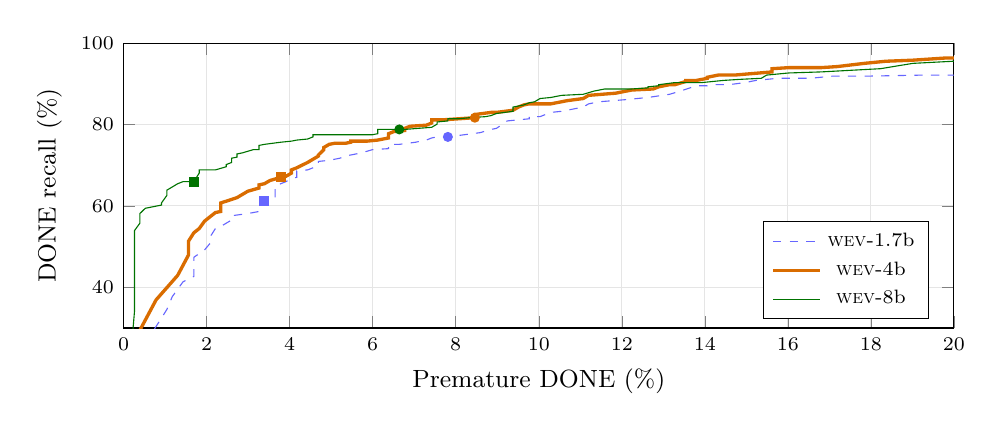
\begin{tikzpicture}
\begin{axis}[width=\linewidth, height=5.2cm, xlabel={Premature DONE (\%)}, ylabel={DONE recall (\%)},
  xmin=0, xmax=20, ymin=30, ymax=100, grid=major, grid style={gray!20}, legend pos=south east,
  legend style={font=\scriptsize}, tick label style={font=\scriptsize}, label style={font=\small}]
\addplot[color=blue!60, dashed] coordinates {(37.63,97.12) (34.90,97.12) (32.68,97.12) (30.47,96.07) (28.39,95.03) (27.08,95.03) (26.56,94.76) (25.78,94.24) (25.39,93.46) (24.48,92.93) (23.57,92.67) (22.92,92.67) (22.53,92.67) (21.88,92.41) (20.44,92.15) (19.27,92.15) (17.84,91.88) (17.06,91.88) (16.54,91.36) (15.76,91.36) (15.23,90.84) (14.97,90.31) (14.58,89.79) (14.19,89.79) (14.06,89.53) (13.80,89.53) (13.41,88.22) (13.15,87.43) (12.63,86.65) (12.11,86.13) (11.46,85.60) (11.46,85.60) (11.20,85.08) (11.07,84.29) (10.81,83.77) (10.55,83.25) (10.29,82.98) (10.03,81.94) (9.77,81.94) (9.77,81.41) (9.24,80.89) (8.98,79.06) (8.85,78.80) (8.59,78.01) (8.20,77.49) (7.81,76.96) (7.55,76.96) (7.42,76.70) (7.42,76.70) (7.29,76.18) (7.16,75.92) (7.03,75.65) (6.64,75.13) (6.38,75.13) (6.38,74.08) (5.99,73.82) (5.73,73.04) (5.34,72.25) (5.21,71.73) (5.21,71.73) (4.95,71.20) (4.69,70.94) (4.69,70.42) (4.69,69.90) (4.56,69.37) (4.43,68.85) (4.17,68.59) (4.17,67.02) (4.04,66.75) (3.91,65.97) (3.65,64.92) (3.65,63.61) (3.65,63.35) (3.65,62.83) (3.65,62.04) (3.39,61.26) (3.39,59.95) (3.26,58.64) (2.99,58.12) (2.60,57.59) (2.60,56.54) (2.34,54.97) (2.21,54.45) (2.08,52.36) (2.08,50.79) (1.95,49.21) (1.69,47.38) (1.69,45.55) (1.69,42.67) (1.43,41.36) (1.17,37.70) (1.04,34.55) (0.65,28.27) (0.39,19.11) (0.00,9.16)};
\addlegendentry{\wev-1.7b}
\addplot[color=orange!85!black, very thick] coordinates {(25.39,97.91) (23.70,97.38) (22.66,96.60) (20.83,96.34) (19.79,96.34) (19.01,95.81) (18.36,95.55) (17.84,95.03) (17.19,94.24) (16.80,93.98) (16.02,93.98) (15.62,93.72) (15.62,92.93) (14.71,92.15) (14.32,92.15) (14.19,91.88) (14.06,91.62) (14.06,91.62) (14.06,91.62) (14.06,91.36) (13.80,90.84) (13.54,90.84) (13.54,90.58) (13.28,89.79) (13.15,89.79) (13.15,89.79) (12.89,89.27) (12.76,88.74) (12.76,88.74) (12.76,88.74) (12.24,88.48) (11.98,87.96) (11.85,87.70) (11.20,87.17) (11.07,86.39) (10.68,85.86) (10.29,85.08) (9.77,85.08) (9.64,84.82) (9.51,84.29) (9.51,84.29) (9.38,83.51) (8.98,82.98) (8.85,82.98) (8.46,82.46) (8.46,81.68) (7.68,81.15) (7.42,81.15) (7.42,80.37) (7.29,79.84) (6.90,79.58) (6.77,79.06) (6.77,78.80) (6.77,78.53) (6.51,78.27) (6.38,77.75) (6.38,76.70) (6.12,76.18) (5.86,75.92) (5.60,75.92) (5.47,75.92) (5.47,75.65) (5.34,75.39) (5.21,75.39) (5.08,75.39) (4.95,75.13) (4.82,74.35) (4.82,73.82) (4.69,72.51) (4.69,72.25) (4.43,70.68) (4.17,69.37) (4.04,68.85) (4.04,68.06) (3.91,67.28) (3.78,67.02) (3.52,66.23) (3.39,65.45) (3.26,65.18) (3.26,64.40) (2.99,63.61) (2.73,62.04) (2.34,60.73) (2.34,59.42) (2.34,58.64) (2.21,58.38) (1.95,56.28) (1.82,54.45) (1.69,53.40) (1.56,51.31) (1.56,47.91) (1.30,42.93) (0.78,36.91) (0.26,26.96) (0.00,14.14)};
\addlegendentry{\wev-4b}
\addplot[color=green!45!black] coordinates {(22.27,96.86) (20.96,96.07) (19.01,95.03) (18.23,93.72) (16.80,92.93) (16.02,92.67) (15.49,92.15) (15.36,91.36) (14.84,91.10) (14.45,90.84) (13.93,90.31) (13.54,90.31) (13.28,90.31) (12.89,89.79) (12.89,89.53) (12.63,89.27) (12.63,89.01) (12.24,88.74) (11.98,88.74) (11.59,88.74) (11.33,88.22) (11.07,87.43) (10.55,87.17) (10.29,86.65) (10.03,86.39) (9.90,85.60) (9.77,85.34) (9.64,84.82) (9.38,84.29) (9.38,84.03) (9.38,83.77) (9.38,83.25) (8.98,82.72) (8.85,82.20) (8.72,81.94) (8.33,81.68) (8.07,81.41) (7.81,81.41) (7.81,80.89) (7.55,80.63) (7.55,80.37) (7.55,80.10) (7.42,79.32) (6.77,78.80) (6.64,78.80) (6.64,78.80) (6.64,78.80) (6.12,78.80) (6.12,77.75) (5.99,77.49) (5.60,77.49) (5.47,77.49) (4.95,77.49) (4.56,77.49) (4.56,76.96) (4.43,76.44) (4.17,76.18) (4.04,75.92) (3.78,75.65) (3.78,75.65) (3.39,75.13) (3.26,74.87) (3.26,74.61) (3.26,73.82) (3.12,73.82) (2.86,73.04) (2.73,72.77) (2.73,71.99) (2.60,71.73) (2.60,70.68) (2.47,70.16) (2.47,69.63) (2.21,68.85) (1.82,68.85) (1.82,68.06) (1.69,65.97) (1.43,65.97) (1.30,65.45) (1.30,65.45) (1.04,63.87) (1.04,63.35) (1.04,62.57) (0.91,60.73) (0.91,60.21) (0.52,59.42) (0.39,58.12) (0.39,57.59) (0.39,55.76) (0.26,53.93) (0.26,51.05) (0.26,47.12) (0.26,44.76) (0.26,40.84) (0.26,34.03) (0.13,18.32)};
\addlegendentry{\wev-8b}
\addplot[only marks, mark=*, mark size=1.6pt, color=blue!60, forget plot] coordinates {(7.81,76.96)};
\addplot[only marks, mark=square*, mark size=1.6pt, color=blue!60, forget plot] coordinates {(3.39,61.26)};
\addplot[only marks, mark=*, mark size=1.6pt, color=orange!85!black, forget plot] coordinates {(8.46,81.68)};
\addplot[only marks, mark=square*, mark size=1.6pt, color=orange!85!black, forget plot] coordinates {(3.78,67.02)};
\addplot[only marks, mark=*, mark size=1.6pt, color=green!45!black, forget plot] coordinates {(6.64,78.80)};
\addplot[only marks, mark=square*, mark size=1.6pt, color=green!45!black, forget plot] coordinates {(1.69,65.97)};
\end{axis}
\end{tikzpicture}
\caption{Stopping trade-off on the NNetNav test split (382 DONE steps, 768 others). Each curve
accepts DONE only when its probability exceeds a threshold swept from 0.05 to 0.99; circles mark 0.5 and squares 0.8.}
\label{fig:done}
\end{figure}
\newcommand{\DONECURVETEXT}{At a threshold of 0.5, \wev-4b recalls 82\% of DONE steps and stops early on 8.5\% of the others; at 0.8 the premature rate falls to 3.8\% while recall falls to 67\%. \wev-8b reaches 1.7\% premature stops at 66\% recall, or 2.9\% at 73\% with a threshold of 0.7. The curves are smooth, so a deployment can choose its operating point from development data rather than accept the most probable operation, which answers DONE whenever it outranks the other seven operations and so behaves like a threshold below 0.5.}


An agent acts on the most probable option, but a calibrated probability lets it act more selectively. The expected
calibration error stays at or below 0.06 on browser steps and at or below 0.10 on out-of-domain decisions
(\cref{tab:calib}). The most consequential browser decision is when to stop: stopping early ends a task unfinished,
and stopping late wastes the budget. \Cref{fig:done} shows the trade-off obtained by accepting DONE only above a
threshold on its probability. \DONECURVETEXT

\subsection{What helped and what did not}
\label{sec:ablation}

\paragraph{The second teacher collection.} Adding 2{,}274 decisions from tasks the first collection had not solved
raised \wev-4b's live-website successes from 21 to 30. Paired by task (\cref{tab:paired}), 10 tasks were gained and 1
was lost, an asymmetry unlikely under run-to-run noise (exact McNemar test, $p=0.012$).

\begin{table}[t]
\centering
\caption{Paired live-website outcomes when the second teacher collection is added. Gained: solved only with it;
lost: solved only without it.}
\label{tab:paired}
\begin{tabular}{lcccc}
\toprule
 & Both & Gained & Lost & Total with \\
\midrule
\wev-4b & 20 & 10 & 1 & 30 \\
\wev-8b & 20 & 8 & 8 & 28 \\
\bottomrule
\end{tabular}
\end{table} Its test accuracy stayed within 0.6 points
on every benchmark. For \wev-8b the same data left live-website successes at 28, with 8 tasks gained and 8 lost, and
lowered transfer-v4 by 1.8 points, so \wev-8b keeps the first mixture.

\paragraph{A second epoch.} Training \wev-4b for two epochs changed development accuracy by less than one point on
every benchmark (transfer-v4 74.6 to 75.1, decision-v7 81.9 to 82.6, typed-decisions 79.7 to 79.2, Mind2Web step
success 80.0 to 79.3) at twice the cost.

\paragraph{Structural variants.} On 1.7B, with an earlier mixture, three seeds and development splits, we tested a set
head, which runs a two-layer permutation-equivariant transformer over the option states before scoring, and truncation
of the backbone to its first 18 of 28 layers. Mind2Web step success was $69.0\pm2.7$ for the pointer head at full
depth, 66.5 for the set head at full depth and $68.5\pm0.2$ for the set head on 18 layers, which ran 23\% faster. A later
control run on identical hardware put the cost of truncation at about three points, and the set head did not help at
full depth, so the released models use the pointer head and every layer.

\subsection{Efficiency}
\label{sec:results-latency}

\begin{table}[t]
\centering
\caption{Median in-process latency on one RTX 5090 (bf16, one request at a time). All questions of a request share one
forward pass.}
\label{tab:latency}
\resizebox{\linewidth}{!}{%
\begin{tabular}{lccc}
\toprule
 & decision-v7 & typed-decisions & Browser step \\
Model & 1 q., 180 tok. & 5 q., 380 tok. & 2 q., 3{,}200 tok. \\
\midrule
\wev-1.7b & 10\,ms & 13\,ms & 91\,ms \\
\wev-4b & 15\,ms & 25\,ms & 217\,ms \\
\wev-8b & 21\,ms & 37\,ms & 322\,ms \\
\bottomrule
\end{tabular}}
\end{table}

Because all questions share one forward pass, five questions cost less than twice one (\cref{tab:latency}), and a
browser step's cost is dominated by encoding the page. On a 16\,GB Apple M5 laptop with the PyTorch MPS backend in
fp32, \wev-1.7b loads in about 30\,s and answers a one-question decision in 77\,ms.

\subsection{Failure analysis}
\label{sec:failure}

\begin{table}[t]
\centering
\caption{Recall of each reference operation on the browser test splits (\%). Rare operations are rarely predicted.}
\label{tab:recall}
\resizebox{\linewidth}{!}{%
\begin{tabular}{llrccc}
\toprule
Split & Operation & Steps & \wev-1.7b & \wev-4b & \wev-8b \\
\midrule
\multirow{3}{*}{Mind2Web} & CLICK & 687 & 96 & 96 & 95 \\
 & SELECT & 65 & 65 & 88 & 88 \\
 & TYPE\_TEXT & 110 & 63 & 75 & 71 \\
\midrule
\multirow{5}{*}{NNetNav} & CLICK & 478 & 82 & 80 & 84 \\
 & DONE & 382 & 80 & 85 & 80 \\
 & TYPE\_TEXT & 201 & 79 & 76 & 76 \\
 & SCROLL (up, down) & 60 & 0 & 0 & 3 \\
 & BLOCKED & 29 & 3 & 3 & 3 \\
\bottomrule
\end{tabular}}
\end{table}

Operations that are rare in training are rarely predicted (\cref{tab:recall}). On NNetNav test steps, recall is 76--85\% for CLICK,
TYPE\_TEXT and DONE but 3\% for BLOCKED (29 steps) and at most 4\% for scrolling (60 steps), for all three sizes. On
Mind2Web, TYPE\_TEXT recall ranges from 63\% (\wev-1.7b) to 75\% (\wev-4b), against 95--96\% for CLICK. Target choice
remains harder on NNetNav (58--61\%) than on Mind2Web (74--81\%), since NNetNav pages come from live exploration and
have longer, noisier element lists. On live tasks, most failures are pages that block automated browsing and tasks
that exceed the action budget.

\section{Discussion}
\label{sec:discussion}

\paragraph{Why the interface is the right place to distil.} A generative agent's supervision lives in its own action
format: tool calls, free text, or coordinates. Converting that format into typed questions requires choosing, for every
step, which options the student should have seen and how to name them, and every such choice can introduce a mismatch
between training and deployment. At the decision interface the agent has already made these choices, so the teacher
and the student see byte-identical requests. The teacher's reasons are discarded, and only the choice is kept, which is
all that a decision model can learn from a hard-labelled step.

\paragraph{What bounds the student.} Interface distillation cannot exceed its teacher on the states the teacher visits,
and the judge only removes the teacher's failures; it does not correct them. The student matches rather than surpasses
its teacher end to end, and its gains from the second collection came from tasks that the first had failed, which
suggests that coverage of hard states, not the number of easy decisions, is what limits the student. The judge is a
second point of failure: it reads a page, not the world, and it can accept a stop on a page that only resembles the
answer.

\section{Limitations}
\label{sec:limitations}

Our live evaluation has 153 tasks on websites that change between runs, which gives wide intervals; we therefore
compare versions with paired tests. Browser targets are chosen among the elements the agent lists, not all elements on
the page, so our Mind2Web numbers are not comparable to its leaderboard. The teacher's labels are hard choices, so the
student learns the teacher's decisions rather than its uncertainty, and interface distillation inherits the teacher's
blind spots; the judge that filters episodes is itself an LLM. Two test reads informed the choice of \wev-8b. We cover
English only and could not compare with the hosted Jev model. Parts of the training data carry their own terms: several
tasksource-jev source tasks are licensed for research only, and the teacher episodes are outputs of qwen3-max.

\section{Conclusion}
\label{sec:conclusion}

The typed interface between an agent and its System One is a supervision channel: logging a prompted LLM behind it on
live websites, and keeping what a judge confirms, yields training data in the decision model's own format. Combined
with converted demonstrations whose stopping labels we audited, this closes the gap that general decision models leave
on browser steps. \wev answers three quarters of steps on unseen websites, stays competitive on general decisions, and
completes as many live tasks as its teacher, locally and in tens to hundreds of milliseconds per decision. Collecting
teacher labels on the states the student itself reaches, in the manner of DAgger \citep{ross2011dagger}, is the
natural next step.

\section*{Impact Statement}

This work makes browser agents cheaper to run and removes their dependence on a hosted decision API, which lowers the
barrier to automating web tasks. Automated browsing can be misused, for example to scrape sites against their terms or
to act on accounts without consent. Our teacher prompt forbids signing in, purchasing, posting, messaging and submitting
personal information, and the student learns to answer BLOCKED on CAPTCHAs and login walls, but these behaviours are
learned, not guaranteed. We release the models as research artifacts under Apache-2.0, note the research-only terms of
part of the training data, and recommend human oversight for any deployment that acts on behalf of users.

\bibliography{refs}
\bibliographystyle{icml2026}

\newpage
\appendix
\onecolumn

\section{Teacher and Judge Prompts}
\label{app:prompts}

\paragraph{Teacher.} The teacher server renders each request as the goal, URL, title, up to 6{,}000 characters of
visible page text, the element list with roles, labels, states and allowed operations, the recent actions, the
operation options with their rubrics, and the valid target keys per operation, followed by the agent's own rules and
these safety rules:
\begin{quote}\small
Never sign in, register, buy, book, pay, post, comment, send messages, or submit personal information. If the next step
would need any of those, a CAPTCHA, an ``unusual traffic'' page, or a login wall: choose BLOCKED. If the goal is already
visibly satisfied: choose DONE. Do not keep browsing after that.
\end{quote}
The teacher replies with a JSON object holding one operation key, one valid target key or null, and a one-sentence
reason.

\paragraph{Judge.} The judge receives the goal and the current browser state and is instructed:
\begin{quote}\small
Decide whether the goal has already been fully achieved, so that the correct next step is to stop and report
completion. ``done'' is true only if the current page and the actions taken already satisfy every part of the goal. For
information-seeking goals, done is true when the requested information is visible on the current page or was clearly
reached by the actions taken. For goals that require an action, done is true only if that action has visibly been
completed. If a required part is missing, or the page does not show the information yet, done is false.
\end{quote}
It replies with a JSON object holding a boolean and a one-sentence reason.

\section{Hyperparameters}
\label{app:hparams}

\begin{table}[h]
\centering
\caption{Training hyperparameters of the released models.}
\small
\begin{tabular}{lccc}
\toprule
 & \wev-1.7b & \wev-4b & \wev-8b \\
\midrule
Base model & Qwen3-1.7B-Base & Qwen3-4B-Base & Qwen3-8B-Base \\
Layers & 28 & 36 & 36 \\
LoRA rank / targets & \multicolumn{3}{c}{16 / all attention and MLP projections} \\
Pointer-head dimension $d_p$ & \multicolumn{3}{c}{256} \\
Peak learning rate, schedule & \multicolumn{3}{c}{$10^{-4}$, one-cycle, 10\% warm-up} \\
Epochs & \multicolumn{3}{c}{1} \\
Padded tokens per micro-batch and GPU & 20{,}000 & 6{,}000 & 6{,}000 \\
GPUs (NVIDIA H20) & 1 & 8 & 8 \\
Training time & 146 min & 66 min & 89 min \\
Teacher collections & first & first and second & first \\
Maximum state / question tokens (inference) & \multicolumn{3}{c}{4{,}096 / 8{,}192} \\
\bottomrule
\end{tabular}
\end{table}

\section{Development Results}
\label{app:dev}

\begin{table}[h]
\centering
\caption{Development results of the \wev-4b candidates (per-question accuracy; browser columns are step success;
Teacher is the development split of the first collection).}
\small
\begin{tabular}{lcccccc}
\toprule
Candidate & decision-v7 & transfer-v4 & typed-dec. & Mind2Web & NNetNav & Teacher \\
\midrule
First collection, 1 epoch & 81.9 & 74.6 & 79.7 & 80.0 & 64.8 & 71.1 \\
First collection, 2 epochs & 82.6 & 75.1 & 79.2 & 79.3 & 67.6 & 69.0 \\
Both collections, 1 epoch (released) & 81.5 & 72.6 & 79.7 & 77.2 & 66.7 & 74.1 \\
\bottomrule
\end{tabular}
\end{table}

\section{Release}
\label{app:release}

Code, data builders and per-request evaluation outputs: \url{https://github.com/alanhuangyoo/wev}. Models:
\url{https://huggingface.co/alanhuangya}. Package: \texttt{pip install wev-ai}.

\end{document}
